\section{Results} 
In this section we present some initial results we
gathered from our preliminary experiments.
We used Apache Storm v$0.9.4$ and Java
OpenJDK v1.7. The topology we utilized in our experiments
consisted of a Relevancy operator, followed by a
Diversity Operator.
As far as our dataset is concerned,
we gathered tweets using Twitter's Streaming API,
and accumulated $75000$ tweets.
Even though the Streaming API provides a
plethora of attributes for each Tweet, we
kept only the creation date and the text.
The reason for that is because those are
the only attributes important for our experiments
(creation date for recency and text for relevance).
During the gathering process, we ignored tweets
that had non-ASCII characters, since those do
not contain usable information and posed
problems in storage.

In order to get a first impression on StreamDiv's
effectiveness, we decided to compare it with the
offline version.
We compare StreamDiv with the offline implementation
of combined relevance-and-diversity, which is named
PrefDiv. The latter performs the same
algorithm, but it reads data from a database
and has a global view of the tweets.
Our experiments were designed in a way to measure
StreamDiv's performance on (i) diversity, (ii) relevance,
and (iii) intensity.

For diversity, we calculated for each pair of tweets
the Cosine Similarity distance. There is no particular
reason that we opted for the previous metric, and the
usage of alternative distances is orthogonal to our
experiments. In terms of relevance, we used a simple
approach, which annotated each tweet with a score,
based on a given set of keywords.
The score is just the number of
keywords found in the text of the tweet.
The result show in figures \ref{fig:avg-distance}, \ref{fig:avg-relevancy}, \ref{fig:norm-intensity}
are based on the statistic of the final top-k list of each model. Hence, for the incremental algorithm the result are constant.

Table \ref{table:par} illustrated different parameters of the experiment, such that $\alpha$ is the scaling factor between relevancy and diversity,
Radius is a parameter that use to distinguish between the similar and dissimilar items, for two tweets that has the cosine similarity larger then Radius 
we consider them as dissimilar.

\begin{table}[!tb] 
\centering
\caption{PARAMETER CONFIGURATION}
\resizebox{0.22\textwidth}{!}{\begin{tabular}{|c|c|} \hline
PARAMETER & VALUE \\ \hline \hline
p & 0.5 \\ \hline
$\alpha$ & 0.5 \\ \hline
Radius & 0.8 \\ \hline
Dataset size & 75000 \\ \hline
\end{tabular}}
\label{table:par}
\end{table}

\begin{figure}[!htb]
\centering
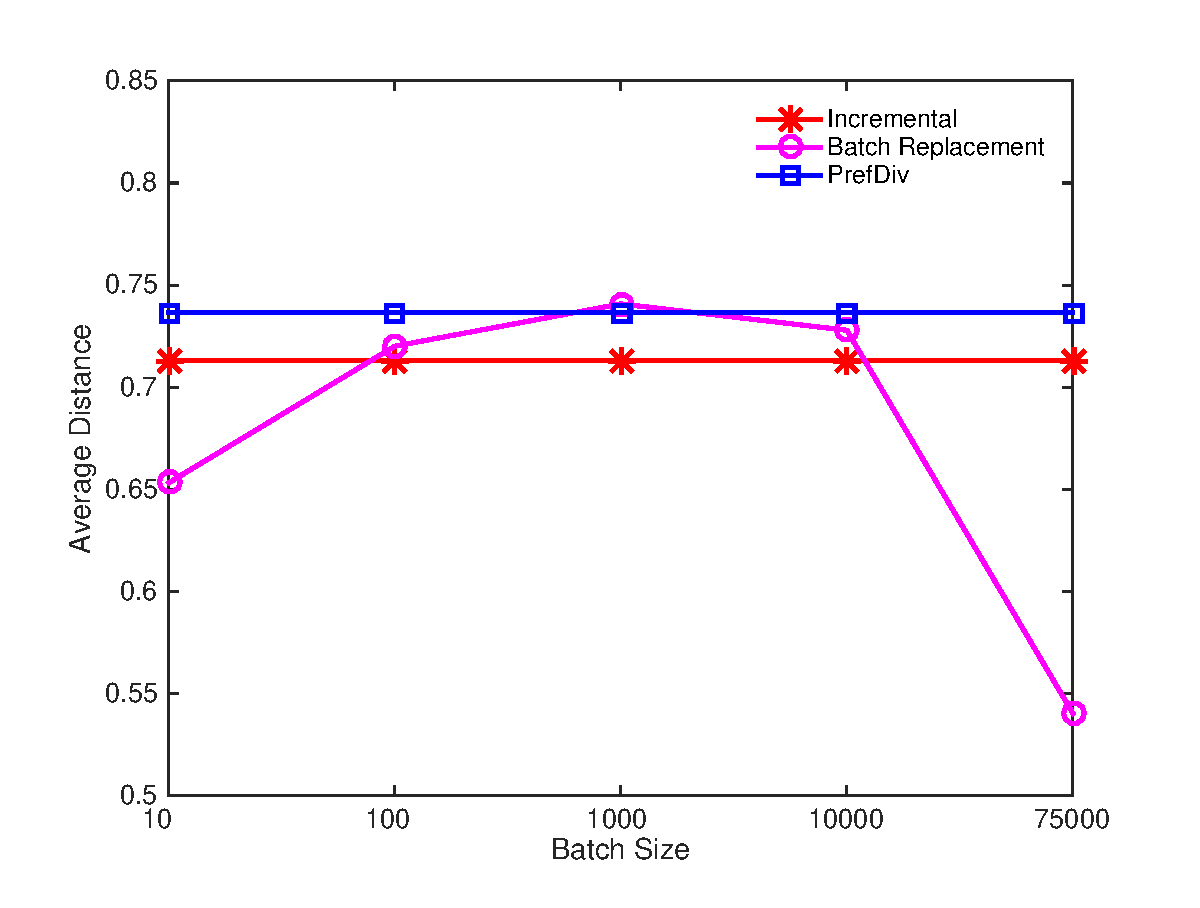
\includegraphics[width=0.4\textwidth,height=0.4\textheight,keepaspectratio]{Figures/AverageDistance.eps}
\caption{Average Distance on different batch windows.}
\label{fig:avg-distance}
\end{figure}

Figure~\ref{fig:avg-distance} depicts the average distance
achieved by using different batch sizes on StreamDiv.
The incremental version of StreamDiv is not affected by
the batch size, because it will always replace the
same percentage of elements on every tuple.
Therefore, the distance remains constant.
The previous happens also in
relevance and intensity.
Turning to the batch version of StreamDiv, it is interesting
how greater batch sizes, produce worse results in terms of diversity.
The degradation of diversity is expected since the replacement
policy of our prototype is naive at this point.
In detail, the same percentage of tuples
is discarded at every epoch. Hence, even if we achieve
higher diversity at some point, a large number of tuples
will be discarded, and the average distance will drop.

\begin{figure}[!htb]
\centering
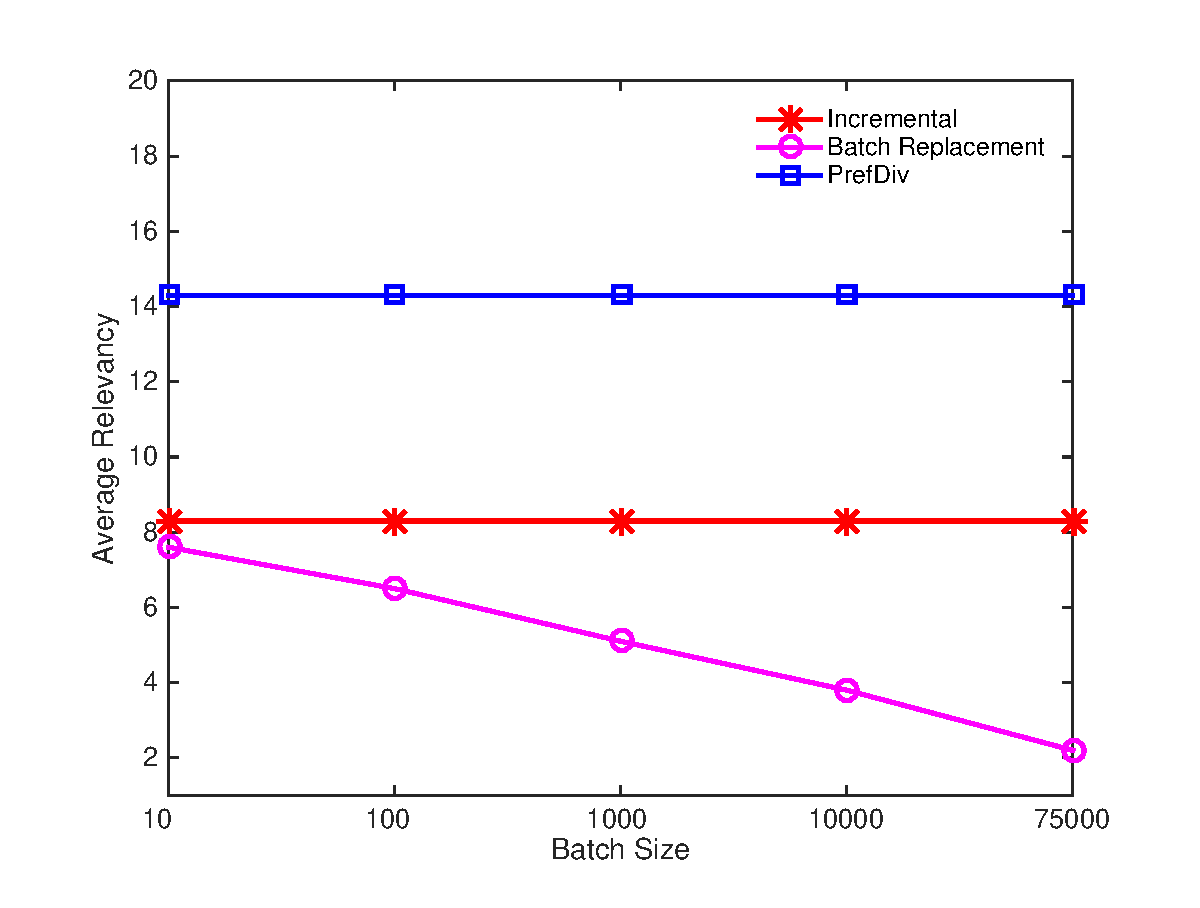
\includegraphics[width=0.4\textwidth,height=0.4\textheight,keepaspectratio]{Figures/AverageRelevancy.eps}
\caption{Average Relevancy on different batch windows.}
\label{fig:avg-relevancy}
\end{figure}

Turning to relevance, we monitored similar results with
average distance (depicted in Fig.~\ref{fig:avg-relevancy}).
The number of tuples that will be replaced
increases with the batch size. Therefore, the batch approach
will more likely throw away important tuples.
The same story appears in normalized intensity (see Figure~\ref{fig:norm-intensity}).
We expect that with the dynamic reconfiguration of the
percentage, we will achieve better results.

\begin{figure}[!htb]
\centering
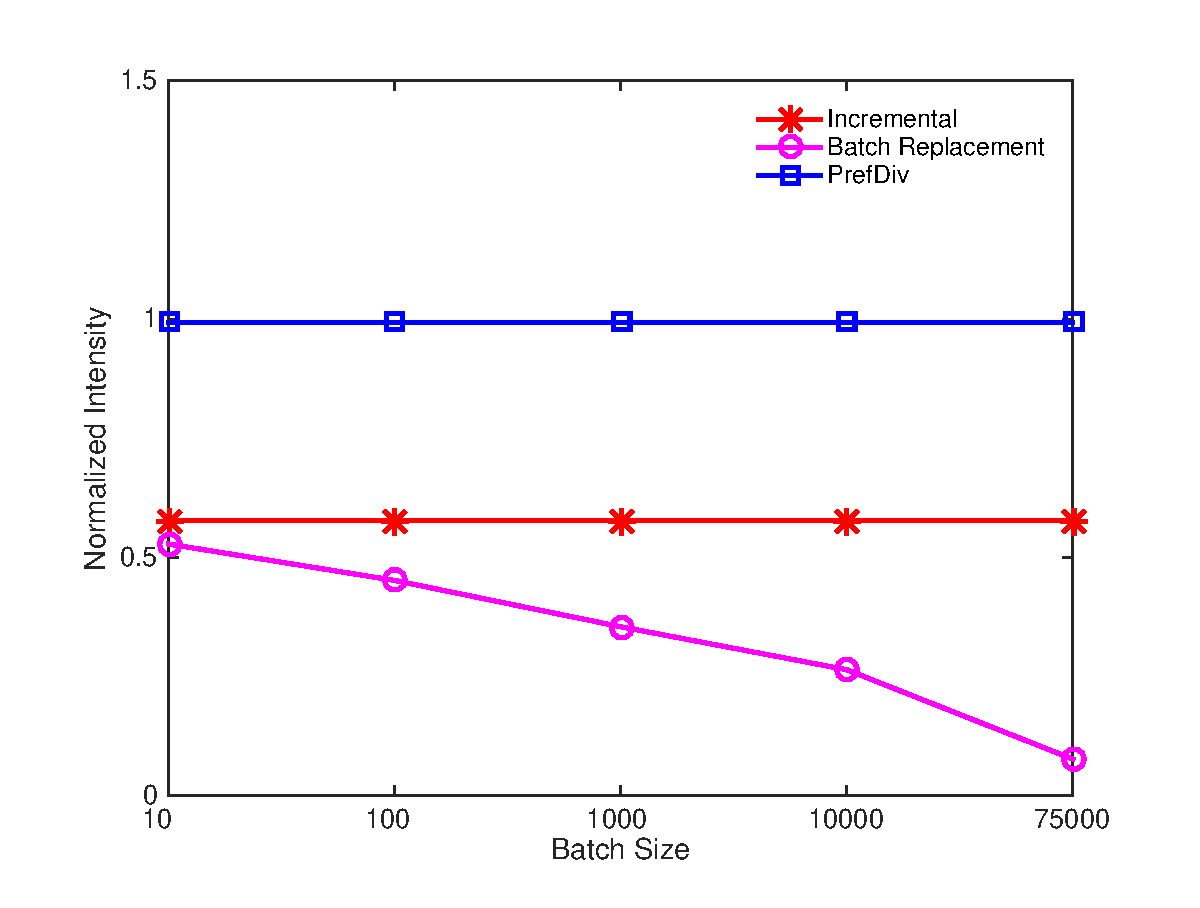
\includegraphics[width=0.4\textwidth,height=0.4\textheight,keepaspectratio]{Figures/NormalizedIntensity.eps}
\caption{Normalized Intensity on different batch windows.}
\label{fig:norm-intensity}
\end{figure}